\section{Feasibility Study of a Pixelated \glsentryshort{lartpc} for the \glsentryshort{dune} \glsentrylong{nd}}
\label{sec:dune-nd_pile-up}

With \AC{} selected as  the \lar{} component of the \dune{} \gls{nd}, there were two main question that needed to be addressed:
\begin{enumerate}
	\item Is a pixelated \lartpc{} feasible?
	\item Can the \lar{} detector handle the high rates?
\end{enumerate}
Number one is addressed in Section~\ref{sec:ac_viper}.
This chapter will address question number two.
More details on \dune{} can be found in Section~\ref{sec:nu-detection_dune} while the proposed \AC{} \lar{} component of the \gls{nd} is described in Section~\ref{sec:dune-nd_ac_nd}.

\begin{figure}[htb]
	\centering
	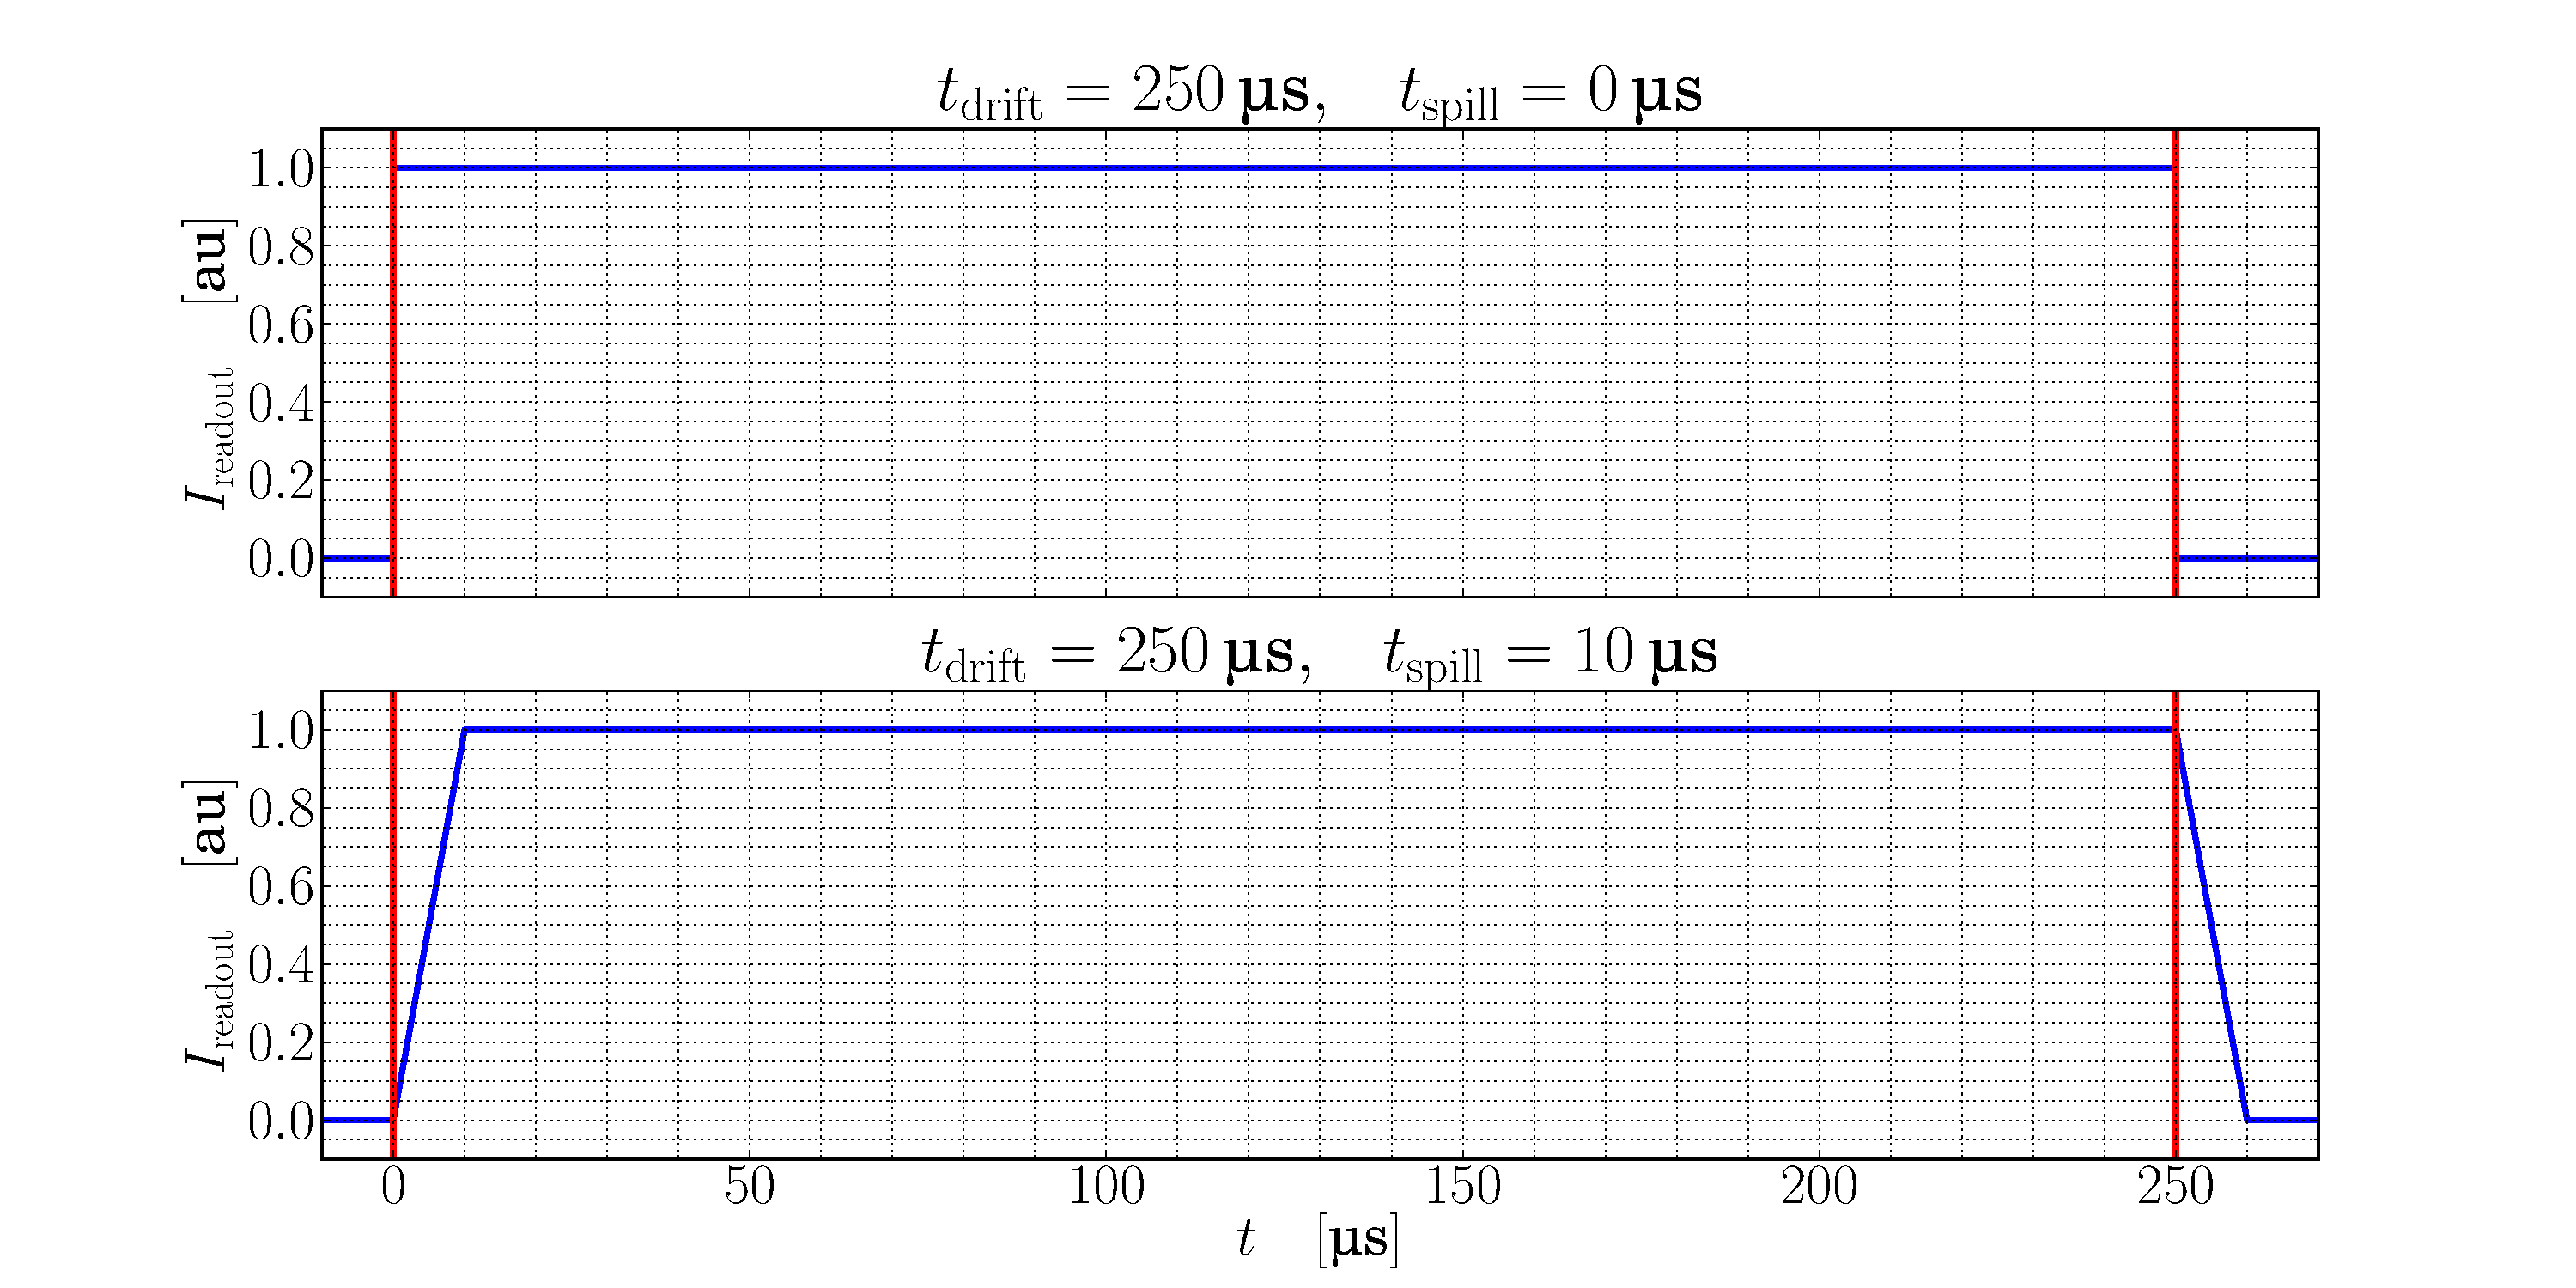
\includegraphics[width=\textwidth]{pile-up/charge_flux}
	\caption{Average current collected by the readout for one spill as a function of time.
	The current is given in arbitrary but equal units for both plots.
	Anode and cathode are represented by the vertical red lines, relative to the trigger timestamp.
	The upper plot assumes the whole charge is deposited instantaneously while for the lower plot, the actual spill duration from~\cite{dune2} is used.}
	\label{fig:dune-nd_charge-flux}
\end{figure}

\lartpc{}s are intrinsically slow detectors with a readout time of $\approx \SI{0.5}{\milli\second\per\metre}$ drift length for a \SI{1}{\kilo\volt\per\centi\metre} drift field (see Chapter~\ref{chap:lartpc}).
This causes a pile-up of events in the detector; if the latter was infinitely fast, all neutrino interactions could be separated in time.
In reality, even the \AC{} \glspl{tpc} with a drift length of only \SI{0.5}{\metre}, corresponding to a full readout cycle of \SI{250}{\micro\second}, are significantly slower than the spill duration of \SI{10}{\micro\second} of the \dune{} beamline reference design.~\cite{dune2}
Figure~\ref{fig:dune-nd_charge-flux} visualises this effect.
The charge arriving at the readout is represented as an average current in arbitrary units (the same for top and bottom, though).
Anode and cathode are represented by the vertical red lines, relative to the trigger timestamp.
The magnitude of the readout current is a direct measure for event pile-up in the corresponding time slice.
For simplicity, an infinitely short spill duration was assumed for the pile-up study (top), i.e.\ the whole ionisation charge produced by one beam spill is deposited instantaneously inside the \gls{tpc} volume.
As the time in between beam spills is $\sim{\SI{1}{\second}}$, all this charge can be read out within one drift time.
In this case, the average current (pile-up) seen by the readout is constant over the whole readout cycle.
The realistic case with the spill duration of the reference beam is depicted in the bottom plot.
At the beginning of the readout cycle, there is no charge deposited yet, the current (pile-up) is zero.
Over the duration of the beam spill, ionisation charge accumulates inside the \gls{tpc} volume while the exisiting charge is transported towards the readout by the drift field.
After the beam spill is over, the remainder of the initial drift volume (\SI{240}{\micro\second}) contains a uniform charge density.
The additional \SI{10}{\micro\second}, now in front of the cathode and part of the next readout cycle, again, contain a ramped charge density with zero charge at the cathode, corresponding to the end of the spill.
In short, a spill duration shorter than but comparable to the drift time results in the shape of the ionisation current (event pile-up) seen over time to become a trapecoid rather than a square.
The integral, i.e.\ the total ionisation charge (deposited energy) is the same but part of it is shifted from the spill time slice to the beginning of the next readout cycle.
Similarly, the peak current (pile-up) is the same, as long as the spill duration is shorter than the drift time.
If the spill duration becomes longer than the drift time, the charge is distributed over more then two readout cycles and the peak current (pile-up) begins to decrease.
Therefore, the assumption of an infinitely short spill is a worst-case scenario slightly improved by the real, finite spill duration.
However, for most of the drift time (\SI{240}{\micro\second}), pile-up is the same.


\subsection{\texorpdfstring{\Pgpz}{Pi0} pile-up simulation}
\label{sec:dune-nd_pile-up_simulation}

One way to assess the performance of an analysis of experimental data is to run it on a simulated dataset.
In the simulation, the quantities to be measured by the experiment are known a priori.
They are called truth information and can be compared to the output of the analysis run on the simulated dataset.

A significant amount of \Pgpz are produced in several resonant and coherent neutrino interactions (see Table~\ref{tab:nu-detection_nd-rates} Section~\ref{sec:nu-detection_interactions} and~\cite{dune2}).
They decay according to
\begin{IEEEeqnarray}{C}
	\HepProcess{\Pgpz \to \Pgg\Pgg}
\end{IEEEeqnarray}
with a branching ratio of \SI{98.8}{\percent}\cite{pdg}.
The photons subsequently produce \gls{em} showers in \lar{} (see Section~\ref{sec:nu-detection_fs}).
At the energies of the \dune{} beam (see Figure~\ref{fig:nu-detection_dune-flux}), most showers do not deposit a homogenous cone of charge but rather a lot of individually resolvable \Pepm tracks.
More importantly, there often are significant gaps in betweend these charge clusters.
A main challenge of shower reconstruction is to associate these well-separated charge blobs to the correct event.
Misidentifications lead to a misreconstruction of the neutrino energy.
The resulting discrepancy to the true neutrino energy has the potential to skew the measured energy spectrum and, thus, influence the oscillation measurements.
The complexity of reconstruction paired with the potential impact on the physics measurements makes photons produced by \Pgpz decays a good sample to study the robustness to pile-up of a pixelated \lartpc{} in the \dune{} \gls{nd} environment.

To simulate the expected neutrino interactions in the \gls{nd}, the Argon Box\footnote{\url{https://github.com/dadwyer/argon_box}} simulation tool was used.
The neutrino group at \gls{lbnl} is developing it with the goal of providing an easy-to-use simulation of particle interactions in the \lar{} component of the \gls{nd}.
Primary particles can either be provided by a particle gun (e.g.\ \Pem, \Pn, \Pp, \Pgmp) or in form of a \emph{HEPEVT} file\footnote{A file format standard for passage of particle events between different simulation tools}.
For this study, \num{6.6e6} neutrino events were produced with the GENIE\footnote{\url{https://genie.hepforge.org}} neutrino event generator.
Secondary particle transport and interaction in Argon Box is performed by Geant4.\footnote{\url{http://geant4.cern.ch}}
Finally, the energy deposition in \lar{} is voxelised and stored together with all the necessary ancillary information about the depositing particle.
The data is stored in the tree format of the ROOT data analysis framework\footnote{\url{https://root.cern}}.
This allows for convenient further processing using ROOT.

\begin{table}[htb]
	\centering
	\caption{Parameters of the \Pgpz pile-up simulation.}
	\label{tab:dune-nd_pile-up-params}
	\begin{tabu} to \textwidth {lSs}
		\toprule
		Parameter &						{Value} &				{Unit} \\
		\midrule
		{X-axis} &						{Drift} &				\\
		{Y-axis} &						{Vertical} &			\\
		{Z-axis} &						{Beam} &				\\
		{Resolution X} &				3 &						\milli\metre \\
		{Resolution Y} &				3 &						\milli\metre \\
		{Resolution Z} &				3 &						\milli\metre \\
		{Target volume X} &				\numrange{-100}{500} &	\centi\metre \\
		{Active volume X} &				\numrange{0}{400} &		\centi\metre \\
		{Fiducial volume X} &			\numrange{30}{370} &	\centi\metre \\
		{Target volume Y} &				\numrange{-100}{350} &	\centi\metre \\
		{Active volume Y} &				\numrange{0}{250} &		\centi\metre \\
		{Fiducial volume Y} &			\numrange{30}{220} &	\centi\metre \\
		{Target volume Z} &				\numrange{-400}{500} &	\centi\metre \\
		{Active volume Z} &				\numrange{0}{500} &		\centi\metre \\
		{Fiducial volume Z} &			\numrange{30}{470} &	\centi\metre \\
		{Detection threshold} &			0.1 &					\mega\electronvolt \\
		{Cone extent} &					10 &				 	X_0 \\
		{Cone aperture (full angle)} &	30 &					\degree \\
		{Cylinder diameter} &			5 &						\centi\metre \\
		{Beam intensity} &				2 &						\mega\watt \\
		\bottomrule
	\end{tabu}
\end{table}

To investigate the effects of pile-up on energy reconstruction, a working reconstruction algorithm is necessary.
However, at the time of writing, official reconstruction tools were only available for \lartpc{}s read out by wire planes.\footnote{\url{http://larsoft.org}}
Therefore, a rather primitive algorithm for true \gls{3d} space points was implemented, under the assumption that a positive outcome of such a pile-up study would imply an even better performance of a more sophisticated reconstruction.
This algorithm is explained in the following, its parameters are listed in Table~\ref{tab:dune-nd_pile-up-params}.

The basic underlying assumption is that a pixel readout without analogue multiplexing will yield unambiguous \gls{3d} space points of charge deposition with a given resolution, depending on the geometry of the pixel plane, time resolution of the readout electronics, and charge transport effects.
Section~\ref{sec:ac_viper} proves that this is feasible provided the current reconstruction ambiguities can eliminated by a successful deployment of the \larpix{} charge readout electronics described in Section~\ref{sec:studies_electronics_pixel}.
The spatial resolution of the pixel readout is assumed to be \SI{0.3}{\centi\metre} based on the \gls{nd} design specified in Section~\ref{sec:dune-nd_ac_nd}\todo{justify!}.
A conservative value of \SI{0.3}{\centi\meter} was chosen in drift direction.
This has several advantages.
Choosing the same resolution as the pixel pitch makes the simulation independent of the orientation of the \gls{tpc}.
\uboone{} has achieved a resolution in drift direction $< \SI{0.3}{\centi\metre}$~\cite{uboone}, making it safe to assume \larpix{} will have a similar performance, even though not yet fully characterised.
Finally, a conservative value also accounts for charge diffusion.
Furthermore, it is assumed that \gls{em} showers can be identified and their starting point and direction reconstructed with negligible errors and inefficiencies, i.e.\ this information is taken from the simulation truth.
In reality, the direction and starting point can be derived from the vertex producing the \Pgpz, and a rough shower direction obtained from a pattern recognition.
A cone is calculated in the direction of the shower with its tip at the first charge deposition of the initial photon.
The opening angle and longituginal extent of the cone were optimised by looking at the distributions of the distance from the starting point and angle w.r.t.\ the direction of the shower.
The finite resolution of the detector is emulated by voxelising (via rounding) the charge deposition with the corresponding resolution in all three spatial coordinates.
This leads to problems near the tip of the cone where the transversal extent is lower than the voxel dimensions.
In particular, it can happen that most of the initial charge is shifted outside the cone.
Furthermore, multiple scattering at lower energies makes the cone model suboptimal near the tip.
Therefore, the acceptance volume for the reconstruction is taken as the union of the cone with a cylinder around the direction of the shower of the same longitudinal extent as the cone.
The cylinder radius was tuned to optimise the trade-off between missed and misidentified energy deposition as defined below.

\begin{figure}[htb]
	\centering
	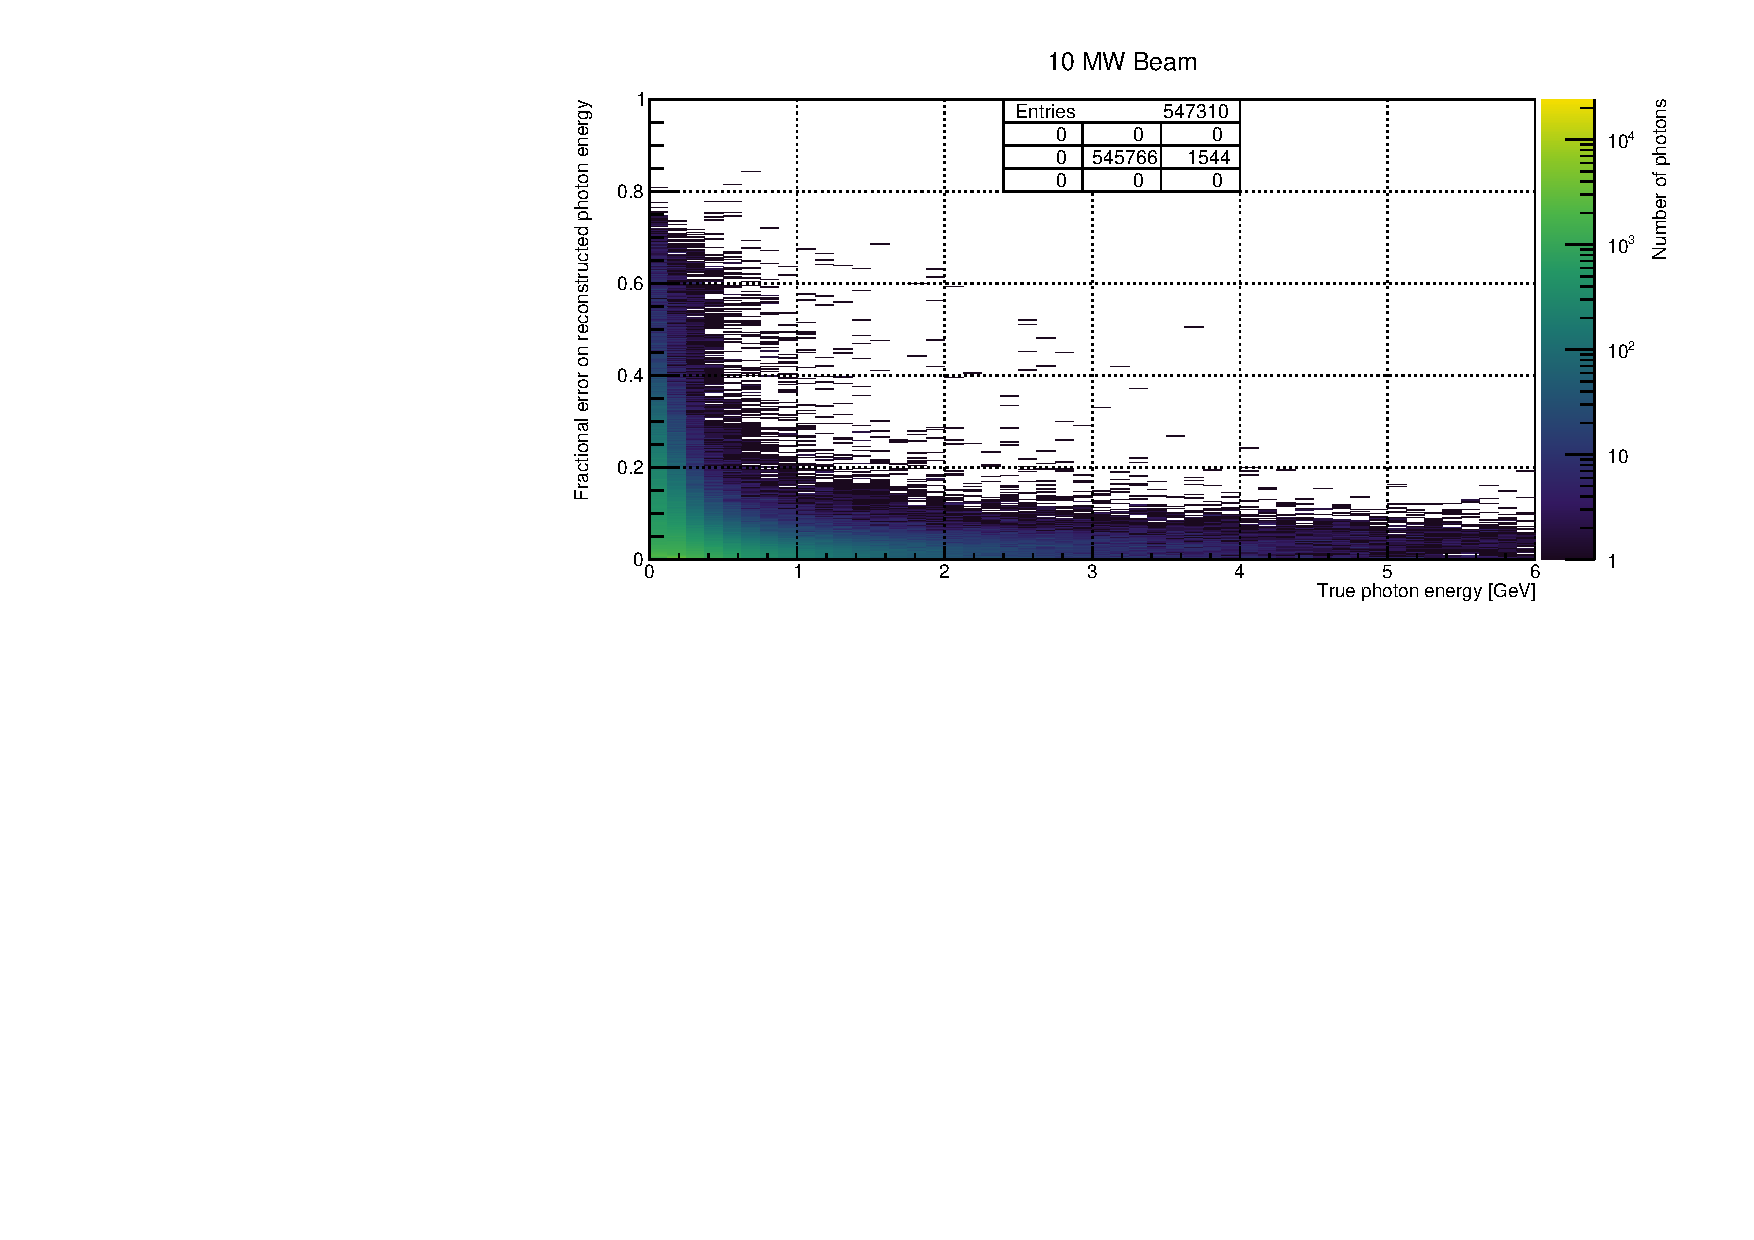
\includegraphics[width=\textwidth]{pile-up/2MW/rel_2d_missed}
	\caption{\gls{2d} histogram of missed energy fraction versus true photon energy for a simple \Pgpz-induced \gls{em} shower reconstruction algorithm based on a cone-cylinder union.
		All energy deposited outside of the cone-cylinder union is counted as missed.
		The simulated beam intensity is \SI{2}{\mega\watt} at \SI{80}{\giga\electronvolt} proton energy.
		Under the number of entries, a detailed list of the number of entries inside (centre) and outside (edges and corners) the depicted area of the histogram is given (under- and overflow).}
	\label{fig:dune-nd_2MW_rel-2d-missed}
\end{figure}

\begin{figure}[htb]
	\centering
	\includegraphics[width=\textwidth]{pile-up/2MW/missed_rel_x}
	\caption{Missed energy fraction versus true photon energy for a simple \Pgpz-induced \gls{em} shower reconstruction algorithm based on a cone-cylinder union.
		All energy deposited outside of the cone-cylinder union is counted as missed.
		The simulated beam intensity is \SI{2}{\mega\watt} at \SI{80}{\giga\electronvolt} proton energy.}
	\label{fig:dune-nd_2MW_missed-rel-x}
\end{figure}

\begin{figure}[htb]
	\centering
	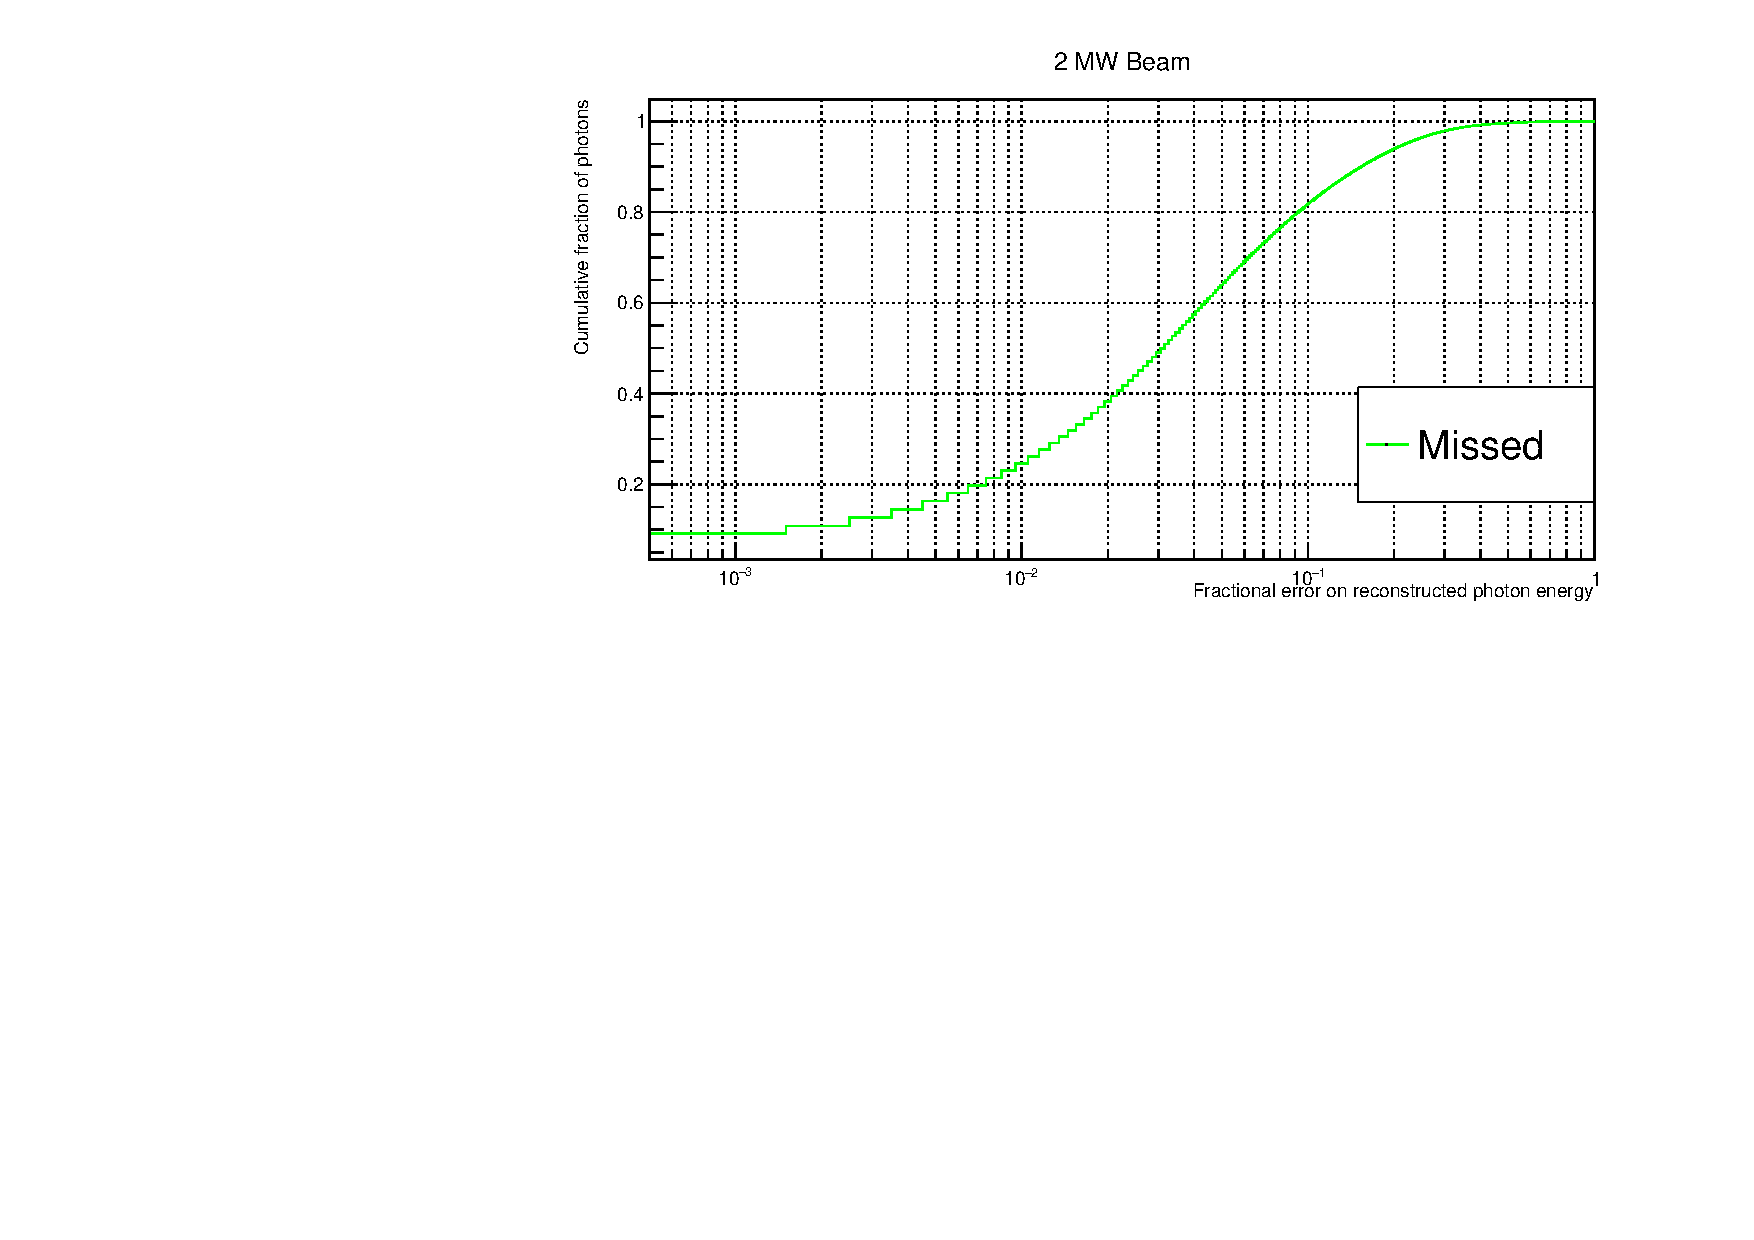
\includegraphics[width=\textwidth]{pile-up/2MW/missed_rel_y}
	\caption{Cumulatetive fraction of photons versus missed energy fraction for a simple \Pgpz-induced \gls{em} shower reconstruction algorithm based on a cone-cylinder union.
		All energy deposited outside of the cone-cylinder union is counted as missed.
		The curve depicts the fraction of photons on the y-axis with a missed energy fraction equal to or lower than the corresponding value on the x-axis.
		The simulated beam intensity is \SI{2}{\mega\watt} at \SI{80}{\giga\electronvolt} proton energy.}
	\label{fig:dune-nd_2MW_missed-rel-y}
\end{figure}

\begin{figure}[htb]
	\centering
	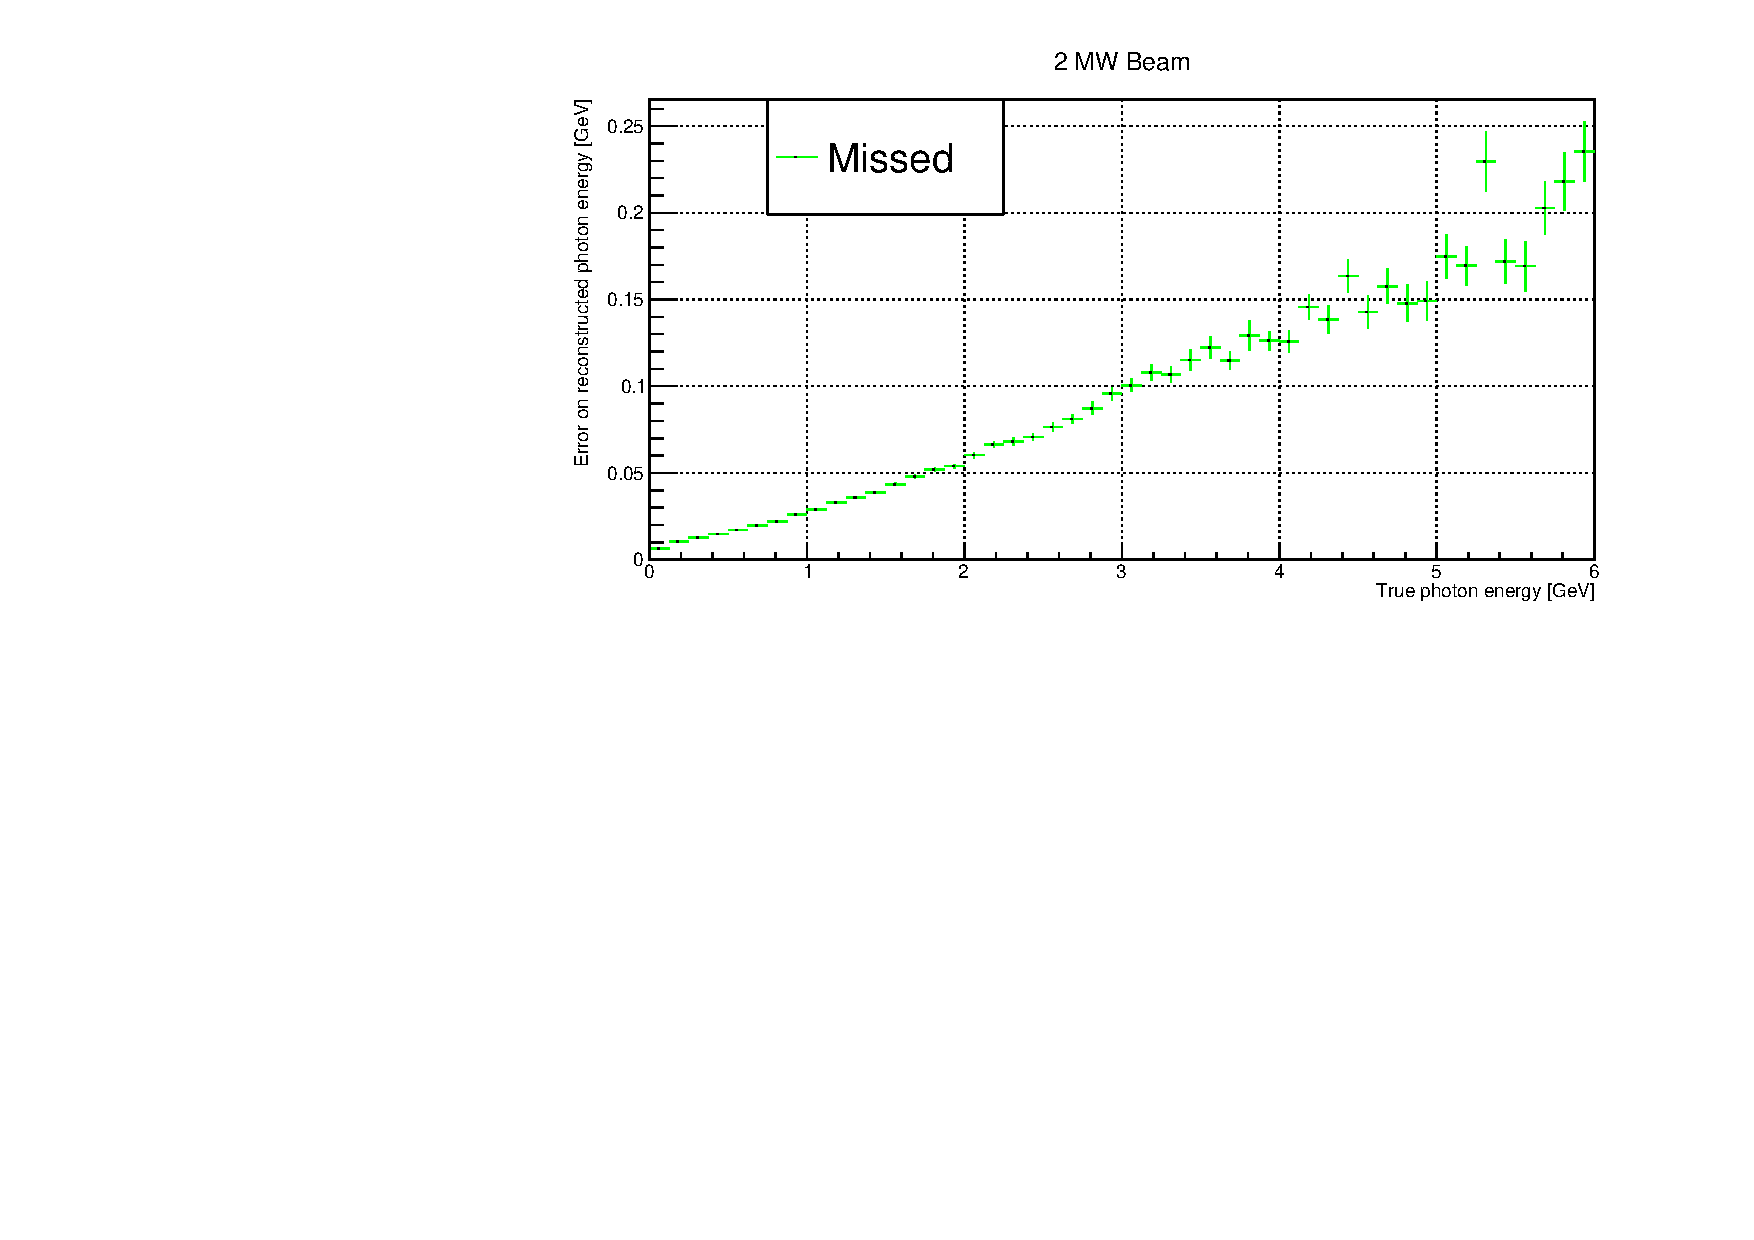
\includegraphics[width=\textwidth]{pile-up/2MW/missed_abs_x}
	\caption{Missed energy versus true photon energy for a simple \Pgpz-induced \gls{em} shower reconstruction algorithm based on a cone-cylinder union.
		All energy deposited outside of the cone-cylinder union is counted as missed.
		The simulated beam intensity is \SI{2}{\mega\watt} at \SI{80}{\giga\electronvolt} proton energy.}
	\label{fig:dune-nd_2MW_missed-abs-x}
\end{figure}

\begin{figure}[htb]
	\centering
	\includegraphics[width=\textwidth]{pile-up/2MW/misid_abs_x}
	\caption{Misidentified energy versus true neutrino energy for a simple \Pgpz-induced \gls{em} shower reconstruction algorithm based on a cone-cylinder union.
		All energy deposited inside the cone-cylinder union by descendants of parent neutrinos different from the parent of the corresponding \Pgpz photon is counted as misidentified.
		Colour indicates different selections of misidentified energy: total (cyan); excluding depositions from muons (red); deposition from photons, neutrons, and their descendants only (blue).
		The simulated beam intensity is \SI{2}{\mega\watt} at \SI{80}{\giga\electronvolt} proton energy.}
	\label{fig:dune-nd_2MW_misid-abs-x}
\end{figure}

\begin{figure}[htb]
	\centering
	\includegraphics[width=\textwidth]{pile-up/2MW/misid_rel_x}
	\caption{Misidentified energy fraction versus true neutrino energy for a simple \Pgpz-induced \gls{em} shower reconstruction algorithm based on a cone-cylinder union.
		All energy deposited inside the cone-cylinder union by descendants of parent neutrinos different from the parent of the corresponding \Pgpz photon is counted as misidentified.
		Colour indicates different selections of misidentified energy: total (cyan); excluding depositions from muons (red); deposition from photons, neutrons, and their descendants only (blue).
		The simulated beam intensity is \SI{2}{\mega\watt} at \SI{80}{\giga\electronvolt} proton energy.}
	\label{fig:dune-nd_2MW_misid-rel-x}
\end{figure}

\begin{figure}[htb]
	\centering
	\includegraphics[width=\textwidth]{pile-up/2MW/misid_rel_y}
	\caption{Cumulative fraction of neutrinos versus misidentified energy fraction for a simple \Pgpz-induced \gls{em} shower reconstruction algorithm based on a cone-cylinder union.
		All energy deposited inside the cone-cylinder union by descendants of parent neutrinos different from the parent of the corresponding \Pgpz photon is counted as misidentified.
		Colour indicates different selections of misidentified energy: total (cyan); excluding depositions from muons (red); deposition from photons, neutrons, and their descendants only (blue).
		The curve depicts the fraction of neutrinos on the y-axis with a misidentified energy fraction equal to or lower than the corresponding value on the x-axis.
		The simulated beam intensity is \SI{2}{\mega\watt} at \SI{80}{\giga\electronvolt} proton energy.}
	\label{fig:dune-nd_2MW_misid-rel-y}
\end{figure}

Argon Box propagates the neutrino interaction events it gets from GENIE through \lar{}, the output is a ROOT tree of neutrino interaction events.
To get a realistic simulation of beam events in the detector, these events need to be distributed randomly in time and space.
Beam spills are simulated by drawing the number of events for each spill from a Poisson distribution whose mean is calculated from the beam intensity and the target mass according to the values in Table~\ref{tab:nu-detection_beam-params}.
The resulting number of events is taken from the Argon Box ROOT tree and their vertices are placed within the \lar{} volume at coordinates drawn from a uniform distribution.
Combined with the target mass given in Table~\ref{tab:dune-nd_pile-up-params}, this results in an equivalent of $\approx \num{1.5e19}$~\gls{pot}.
The seemingly low number (compared to Table~\ref{tab:nu-detection_nd-rates} for instance) is the result of many neutrino interactions happening outside of the active detector.

Three different argon volumes are assumed for the simulation: target, active, and fiducial volume.
The actual detector dimensions are represented by the active volume.
It is inside the target volume which is the volume within which the neutrino vertices are placed randomly.
This is done as a crude emulation of rock events, secondary particles from beam neutrino interactions outside the detector volume.
The additional target mass is \SI{1}{\metre} in all four directions transverse to the beam, and \SI{4}{\metre} in upstream beam direction.
According to Equations~\eqref{eq:nu-detection_hardon-long} and~\eqref{eq:nu-detection_hardon-trans}, hadronic showers up to \SI{10}{\giga\electronvolt} are contained $> \SI{95}{\percent}$ longitudinally and $> \SI{50}{\percent}$ transversally (because Equation~\eqref{eq:nu-detection_hardon-trans} gives the radius for \SI{95}{\percent} containment) in the additional volume.
Or in other words, increasing the target volume further will not result in significantly more rock events entering the active volume.
For transversal containment, it is enough to use the radius for \SI{95}{\percent} containment because the location of the shower is defined by its centre, i.e.\ showers further away than one \SI{95}{\percent} radius from the detector only deposit a minimal amount of energy inside the latter.
These numbers are supported by Geant4 simulations~\cite{hardonContChris}.
As mentioned in Section~\ref{sec:nu-detection_fs}, \gls{em} interactions happen on smaller scales than hadronic interactions.
The big exception are muons due to their high range.
However, as will be explained below, it makes sense to ignore pile-up from muons anyway due to their high reconstruction efficiency.
Finally, a fiducial volume \SI{30}{\centi\metre} ($\approx 2 X_{\m{0}}$) smaller than the active volume on all six faces is defined.
Without the latter, there is a significant number of photons produced by \Pgpz decays inside the detector but only showering outside the detector.
This selection results in $\approx \num{5.5e5}$ processed \Pgpz photons from the initial \num{6.6e6} neutrino events.
Table~\ref{tab:dune-nd_pile-up-params} contains a summary of all the \lar{} volume dimensions.

Active volume dimensions are taken from the preliminary \dune{} \gls{nd} design described in Section~\ref{sec:dune-nd_ac_nd}.
Note that the height was taken as \SI{2.5}{\metre} as opposed to the \SI{3}{\metre} of the \gls{nd} design.
The reason is that another \SI{0.5}{\metre} safety margin were added after this pile-up simulation had been completed.
However, the influence on the pile-up study should be negligible.
The hadron containment studies described in Section~\ref{sec:dune-nd_ac_nd} indicated that \SI{2.5}{\metre} height is the bare minimum.
A safety margin was added to account for unknown uncertainties in the simulation.
However, the same simulation framework was used for both the containment and the pile-up study.
Therefore, the \SI{2.5}{\metre} height is sufficient for the pile-up study.

After all events of one spill are placed inside the target volume, all \Pgpz photons produced inside the fiducial volume are reconstructed using the cone algorithm.
All energy depositions inside the active volume are considered.
To assess the performance of the algorithm and the influence of pile-up on neutrino energy reconstruction, the following two errors on the reconstructed energy are calculated for each \Pgpz photon:
\begin{description}
	\item[Missed energy] is the energy deposited by the corresponding \Pgpz photon (or its descendants) that is outside of the cone-cylinder union and therefore ``missed'' by the algorithm.
		This is a measure of the reconstruction performance and can be used to ensure optimum tuning of the union parameters.
	\item[Misidentified energy] is the energy inside the cone-cylinder union deposited by descendants of a different (``wrong'') parent neutrino.
		This is a measure of event pile-up: the higher the charge deposition by other events inside the union, the higher the event pile-up.
\end{description}
Using this general definition of misidentified energy leads to quite mediocre results.
However, there are some assumptions that can be taken even without knowing the actual reconstruction algorithm.
From results of earlier experiments~\cite{pandora}, the muon reconstruction can be assumed to be very efficient.
Assuming \SI{100}{\percent} reconstruction efficiency for muons and \SI{0}{\percent} for all other particles can therefore serve as an upper limit for misidentified energy.
It can be calculated by ignoring energy deposited by muons originating from other parent neutrinos.
On the other hand, a lower limit for misidentified energy can be calculated by assuming \SI{100}{\percent} reconstruction efficiency for all charged particles and \SI{0}{\percent} for neutral particles (\Pgpz and \Pgg).
This is calculated by only taking into account misidentified energy deposited by neutral particles.
Even assuming \SI{0}{\percent} reconstruction efficiency for neutral particles is potentially too pessimistic.
Future, more sophisticated reconstruction algorithms (e.g. based on machine learning) might be able to partially reconstruct the topology of charge depositions originating from neutral particles and thus prevent their misidentification.
Therefore, it can be assumed that the actual pile-up-related energy reconstruction error is closer to the lower limit and potentially even below.
It should be noted that the upper limit excludes only energy deposited by muons directly and not by their descendants (e.g.\ $\delta$ rays or Michel electrons).
Whereas the lower limit excludes charge deposited by photons, neutrons, and any of their descendants.

\subsection{Results}
\label{sec:dune-nd_pile-up_results}

\begin{figure}[htb]
	\centering
	\includegraphics[width=\textwidth]{pile-up/2MW_XZ/missed_rel_x}
	\caption{Missed energy fraction versus true photon energy for a simple \Pgpz-induced \gls{em} shower reconstruction algorithm based on a cone-cylinder union.
		All energy deposited outside of the cone-cylinder union is counted as missed.
		The simulated beam intensity is \SI{2}{\mega\watt} at \SI{80}{\giga\electronvolt} proton energy.
		As a primitive simulation of a wire readout, only X and Z coordinates are used for the energy reconstruction.}
	\label{fig:dune-nd_2MW-XZ_missed-rel-x}
\end{figure}

\begin{figure}[htb]
	\centering
	\includegraphics[width=\textwidth]{pile-up/2MW_XZ/misid_abs_x}
	\caption{Misidentified energy versus true neutrino energy for a simple \Pgpz-induced \gls{em} shower reconstruction algorithm based on a cone-cylinder union.
		All energy deposited inside the cone-cylinder union by descendants of parent neutrinos different from the parent of the corresponding \Pgpz photon is counted as misidentified.
		Colour indicates different selections of misidentified energy: total (cyan); excluding depositions from muons (red); deposition from photons, neutrons, and their descendants only (blue).
		The simulated beam intensity is \SI{2}{\mega\watt} at \SI{80}{\giga\electronvolt} proton energy.
		As a primitive simulation of a wire readout, only X and Z coordinates are used for the energy reconstruction.}
	\label{fig:dune-nd_2MW-XZ_misid-abs-x}
\end{figure}

\begin{figure}[htb]
	\centering
	\includegraphics[width=\textwidth]{pile-up/2MW_XZ/misid_rel_x}
	\caption{Misidentified energy fraction versus true neutrino energy for a simple \Pgpz-induced \gls{em} shower reconstruction algorithm based on a cone-cylinder union.
		All energy deposited inside the cone-cylinder union by descendants of parent neutrinos different from the parent of the corresponding \Pgpz photon is counted as misidentified.
		Colour indicates different selections of misidentified energy: total (cyan); excluding depositions from muons (red); deposition from photons, neutrons, and their descendants only (blue).
		The simulated beam intensity is \SI{2}{\mega\watt} at \SI{80}{\giga\electronvolt} proton energy.
		As a primitive simulation of a wire readout, only X and Z coordinates are used for the energy reconstruction.}
	\label{fig:dune-nd_2MW-XZ_misid-rel-x}
\end{figure}

\begin{figure}[htb]
	\centering
	\includegraphics[width=\textwidth]{pile-up/2MW_XZ/misid_rel_y}
	\caption{Cumulative fraction of neutrinos versus misidentified energy fraction for a simple \Pgpz-induced \gls{em} shower reconstruction algorithm based on a cone-cylinder union.
		All energy deposited inside the cone-cylinder union by descendants of parent neutrinos different from the parent of the corresponding \Pgpz photon is counted as misidentified.
		Colour indicates different selections of misidentified energy: total (cyan); excluding depositions from muons (red); deposition from photons, neutrons, and their descendants only (blue).
		The curve depicts the fraction of neutrinos on the y-axis with a misidentified energy fraction equal to or lower than the corresponding value on the x-axis.
		The simulated beam intensity is \SI{2}{\mega\watt} at \SI{80}{\giga\electronvolt} proton energy.
		As a primitive simulation of a wire readout, only X and Z coordinates are used for the energy reconstruction.}
	\label{fig:dune-nd_2MW-XZ_misid-rel-y}
\end{figure}

\begin{figure}[htb]
	\centering
	\includegraphics[width=\textwidth]{pile-up/10MW/missed_rel_x}
	\caption{Missed energy fraction versus true photon energy for a simple \Pgpz-induced \gls{em} shower reconstruction algorithm based on a cone-cylinder union.
		All energy deposited outside of the cone-cylinder union is counted as missed.
		The simulated beam intensity is \SI{10}{\mega\watt} at \SI{80}{\giga\electronvolt} proton energy.}
	\label{fig:dune-nd_10MW_missed-rel-x}
\end{figure}

\begin{figure}[htb]
	\centering
	\includegraphics[width=\textwidth]{pile-up/10MW/misid_abs_x}
	\caption{Misidentified energy versus true neutrino energy for a simple \Pgpz-induced \gls{em} shower reconstruction algorithm based on a cone-cylinder union.
		All energy deposited inside the cone-cylinder union by descendants of parent neutrinos different from the parent of the corresponding \Pgpz photon is counted as misidentified.
		Colour indicates different selections of misidentified energy: total (cyan); excluding depositions from muons (red); deposition from photons, neutrons, and their descendants only (blue).
		The simulated beam intensity is \SI{10}{\mega\watt} at \SI{80}{\giga\electronvolt} proton energy.}
	\label{fig:dune-nd_10MW_misid-abs-x}
\end{figure}

\begin{figure}[htb]
	\centering
	\includegraphics[width=\textwidth]{pile-up/10MW/misid_rel_x}
	\caption{Misidentified energy fraction versus true neutrino energy for a simple \Pgpz-induced \gls{em} shower reconstruction algorithm based on a cone-cylinder union.
		All energy deposited inside the cone-cylinder union by descendants of parent neutrinos different from the parent of the corresponding \Pgpz photon is counted as misidentified.
		Colour indicates different selections of misidentified energy: total (cyan); excluding depositions from muons (red); deposition from photons, neutrons, and their descendants only (blue).
		The simulated beam intensity is \SI{10}{\mega\watt} at \SI{80}{\giga\electronvolt} proton energy.}
	\label{fig:dune-nd_10MW_misid-rel-x}
\end{figure}

\begin{figure}[htb]
	\centering
	\includegraphics[width=\textwidth]{pile-up/10MW/misid_rel_y}
	\caption{Cumulative fraction of neutrinos versus misidentified energy fraction for a simple \Pgpz-induced \gls{em} shower reconstruction algorithm based on a cone-cylinder union.
		All energy deposited inside the cone-cylinder union by descendants of parent neutrinos different from the parent of the corresponding \Pgpz photon is counted as misidentified.
		Colour indicates different selections of misidentified energy: total (cyan); excluding depositions from muons (red); deposition from photons, neutrons, and their descendants only (blue).
		The curve depicts the fraction of neutrinos on the y-axis with a misidentified energy fraction equal to or lower than the corresponding value on the x-axis.
		The simulated beam intensity is \SI{10}{\mega\watt} at \SI{80}{\giga\electronvolt} proton energy.}
	\label{fig:dune-nd_10MW_misid-rel-y}
\end{figure}

Missed and misidentified energy by the cone-cylinder union are plotted as a function of true photon and neutrino energy, respectively.
As mentioned above, the missed energy is used to measure the performance of the employed photon reconstruction algorithm.
Therefore, it is sensible to compare it to the true photon energy rather than the true energy of its parent neutrino.
On the other hand, the primary goal of this study is to assess the effect of event pile-up on the neutrino energy spectrum.
The misidentified energy is thus compared to the true neutrino energy.
For this, the total missed energy of each neutrino event is first calculated by summing up the contributions of all descending \Pgpz photons.
Additionally, it is illustrative to look at the fraction of events with a certain misidentified or missed energy.
All the aforementioned information is contained in \gls{2d} histograms of all events with the true neutrino (photon) energy on one axis and the misidentified (missed) energy on the other axis.
The energy dependence of the error can be obtained by looking at the true energy axis and calculating the mean misidentified (missed) energy for each bin (a profile of the \gls{2d} histogram).
Looking at the misidentified (missed) energy axis and summing over all true energy bins yields the number of events with the corresponding misidentified (missed) energy (a projection of the \gls{2d} histogram).
The corresponding fraction of events is obtained by normalising the histogram, i.e.\ dividing every bin by the total number of entries.
It should be noted that for the projections all values in the corresponding y-bin are taken into account, including the ones outside the boundaries of the histogram (under- and overflow).
For the profiles, only events between \SIrange{0}{6}{\giga\electronvolt} absolute and \numrange{0}{1} fractional are taken into account.

The results for a \SI{2}{\mega\watt} beam at \SI{80}{\giga\electronvolt} proton energy are shown in Figures~\ref{fig:dune-nd_2MW_rel-2d-missed} through~\ref{fig:dune-nd_2MW_misid-rel-y}.
To illustrate the relation between the different histograms, all of them are shown for the missed energy in Figures~\ref{fig:dune-nd_2MW_rel-2d-missed} through~\ref{fig:dune-nd_2MW_missed-rel-y}.
The initial \gls{2d} histogram is shown in Figure~\ref{fig:dune-nd_2MW_rel-2d-missed}.
Note that it actually depicts the missed photon energy as a fraction of the true photon energy rather than an absolute value.
Figure~\ref{fig:dune-nd_2MW_missed-rel-x} is the profile of the x-axis, i.e.\ the mean missed energy fraction for each true energy bin.
The projection of the y-axis is depicted in Figure~\ref{fig:dune-nd_2MW_missed-rel-y}.
This is the fraction of photons with a certain missed energy.
It is drawn as a cumulative fraction which means that the curve represents the fraction of photons on the y-axis with a missed energy fraction equal to or lower than the corresponding value on the x-axis.
A consequence of this is that the curve monotonically approaches one towards the right, \SI{100}{\percent} of the reconstructed photons have a missed energy fraction of \SI{100}{\percent} or less.
For reference, Figure~\ref{fig:dune-nd_2MW_missed-abs-x} shows the mean absolute missed energy per true energy bin.

It can be seen that the absolute missed energy rises more or less linearly with the true energy (Figure~\ref{fig:dune-nd_2MW_missed-abs-x}).
This indicates that the cone models the shower well, as expected from theory (see Section~\ref{sec:nu-detection_fs}).
Indeed, it can be seen from Figure~\ref{fig:dune-nd_2MW-XZ_misid-rel-x} that the missed energy stays almost constant at \SI{3}{\percent} from \SIrange{1}{6}{\giga\electronvolt}.
Below, it rises up to \SI{10}{\percent} in the lowest energy bin (\SIrange{0}{125}{\mega\electronvolt}).
This can be explained by the increase in multiple Coulomb scattering at lower momenta.
Similarly, the Compton scattering cross-section increases as well.
Both these effects lead to a higher angular distribution of the energy depositions by electrons (and positrons) and photons, respectively.
Consequentially, more energy is missed because the cone angle is independent of energy.
From Figure~\ref{fig:dune-nd_2MW_missed-rel-y}, it can be seen that for roughly half of the photons, \SI{3}{\percent} of the energy is missed, indicating a symmetric distribution of missed energy around the mean value.
It should be noted that energy deposited outside the detector, so-called leakage, is included in the missed energy.
Despite the fiducial volume, some events still exit the detector.

The behaviour of the misidentified energy is almost opposite to the missed energy: The absolute energy is almost constant with the true neutrino energy (Figure~\ref{fig:dune-nd_2MW_misid-abs-x}), while the fraction of the total energy is inversely proportional to the true energy, accordingly (Figure~\ref{fig:dune-nd_2MW_misid-rel-x}).
Again this is expected as the amount of charge deposited inside the cone originating from other neutrinos should only depend on the geometry of the acceptance volume (i.e.\ the parameters of the cone-cylinder union) and on the event rate but not on the true energy of the reconstructed photon or its parent neutrino.
Also, the effect of the different selections can be seen well.
As mentioned above, the actual error on the reconstructed neutrino energy is probably somewhere in between the red curve, only rejecting misidentified energy deposited by muons, and the dark blue curve, rejecting all but misidentified energy deposited by photons and neutrons or any of their descendants.
From Figure~\ref{fig:dune-nd_2MW_misid-rel-x}, this can be determined to be about \SI{2}{\percent} at the flux peak ($\approx \SI{3}{\giga\electronvolt}$, see Figure~\ref{fig:nu-detection_dune-flux}).
The cumulative neutrino fraction versus the misidentified energy fraction reveals another interesting fact.
It can be seen that about \SI{70}{\percent} of the events experience a pile-up-related error on reconstructed neutrino energy of \SI{1}{\percent} or less.
For roughly \SI{50}{\percent} of the events, it is even below \SI{0.1}{\percent}.
If it was possible to identify the other \SI{50}{\percent} somehow in the real experiment, they could be ignored, giving an essentially pile-up-free sample.
Given the high event rates in the \gls{nd}, this would be easily affordable.
Using the cone-base algorithm described here, \gls{em} shower pile-up could be detected via overlapping cones for instance.

To get a rough idea of the performance of a \gls{2d} wire readout in an identical environment, the same study was performed ignoring the Y-coordinate completely, leaving everything else untouched.
Of course, this is a gross underestimation of the capabilities of existing reconstruction algorithms for \gls{2d} charge readout data.
In particular, contemporary experiments use at least three \gls{2d} projections whereas only one was used here.
Even though, doing this comparison serves to show that the simple cone-cylinder union reconstruction algorithm breaks down for two dimensions as can be seen in Figures~\ref{fig:dune-nd_2MW-XZ_missed-rel-x} through~\ref{fig:dune-nd_2MW-XZ_misid-rel-y}.
The fraction of events not suffering from pile-up is below \SI{10}{\percent}, and \SI{50}{\percent} have \SI{10}{\percent} or more misidentified energy (Figure~\ref{fig:dune-nd_2MW-XZ_misid-rel-y}).
Similarly, the error on energy reconstruction has increased to \SIrange{10}{20}{\percent} at the flux peak (Figure~\ref{fig:dune-nd_2MW-XZ_misid-rel-x}).
On the other hand, the error due to missed energy has improved from \SIrange{3}{2}{\percent} compared to \gls{3d} (Figure~\ref{fig:dune-nd_2MW-XZ_missed-rel-x}).
An explanation for this is that all the energy in Y-direction was summed up, due to the projection on XZ.
Therefore, the cone (or rather triangle) cannot miss energy in the former direction.

Finally, as a cross-check, the (\gls{3d}) pile-up study was performed for a hypothetical \SI{10}{\mega\watt} beam in Figures~\ref{fig:dune-nd_10MW_missed-rel-x} through~\ref{fig:dune-nd_10MW_misid-rel-y}.
As explained above the missed energy only depends on the geometry of the acceptance volume, in particular, it should be independent of beam intensity.
Therefore it is expected to be very similar to the \SI{2}{\mega\watt} case as can be confirmed by comparing Figure~\ref{fig:dune-nd_10MW_missed-rel-x} to Figure~\ref{fig:dune-nd_2MW_missed-rel-x}.
As expected, the error due to misidentified energy is increased to \SIrange{7}{15}{\percent} at the flux peak (Figure~\ref{fig:dune-nd_10MW_misid-rel-x}) but still better than for the XZ projection.
Similarly, only about \SI{10}{\percent} of the neutrino events remain pile-up free, and \SI{50}{\percent} suffer from more than \SI{4}{\percent} misidentified energy (Figure~\ref{fig:dune-nd_10MW_misid-rel-y}).

In summary, this study shows that even a very primitive \gls{em} shower reconstruction algorithm, employing a cone-cylinder union selection, performs well in the high-multiplicity environment of the \dune{} \gls{nd}, when fed with unambiguous \gls{3d} spatial coordinates of energy depositions.
It clearly fails when reduced to two dimensions or presented with a much higher beam intensity.